
\subsection{Differences of the fit between null model and alternative models}

After having fitted all of the models for each of the languages, one of the aspects that we can be wondering about is whether these more complicated alternative models show any difference with respect to the basic linear model: $\langle  d \rangle = f(n) = \frac{n}{3} + \frac{1}{3}$ proposed as null model. 

By visually checking the fit of all the models together in the appendix \ref{appendix:plots}, it can be observed that for all of the languages we can observe a significative difference between the fits of the null hypothesis model (painted in gray color) and the alternative models. The null hypothesis model overestimates by far the value of the function $\langle  d \rangle$ for all the $n$ values, except when $n=2$, that $\langle  d \rangle = 1$, which holds for all the languages.

Similarly, when analyzing the error metric tables, both in the AIC (Tables \ref{tab:aic} and \ref{tab:aic_diff}) and in the residual standard error case (Table \ref{tab:res_se}), the same phenomena can be seen for all of the languages. In the case of the residual standard error metric it was obtained around one order of magnitude more of error value for the null hypothesis model with respect to the alternative models errors. Similarly, way larger values of the AIC metric error were obtained for the null hypothesis model.

\subsection{Best function fit discussion}\label{discussion:bestfit}

One of the questions that arises when visually checking the model plots and the fit of the selected as best model is if this is really the function that provides the best fit for the data. 

It is clear that in terms of the error metrics that were proposed, it is the best fit. But when visually checking, for some of the languages, it can be seen that there are other models that apparently could provide a better fit.

Examining Figure \ref{fig:czech}, one could think that the model is not accurately fitted because the model is far from the mean length when the number of vertices is low (Figure \ref{fig:czech_best_aic}). This can be attributed to the fact that the densities of entries for the number of vertices are not uniform, thus making it more likely to fit better in areas with a higher concentration of entries. Moreover, when the number of vertices is high, the error is greater than when it is low, so our method will attempt to reduce the error for a larger number of vertices.

\begin{figure}[!htb]
    \centering
    \begin{subfigure}{0.4\textwidth}
        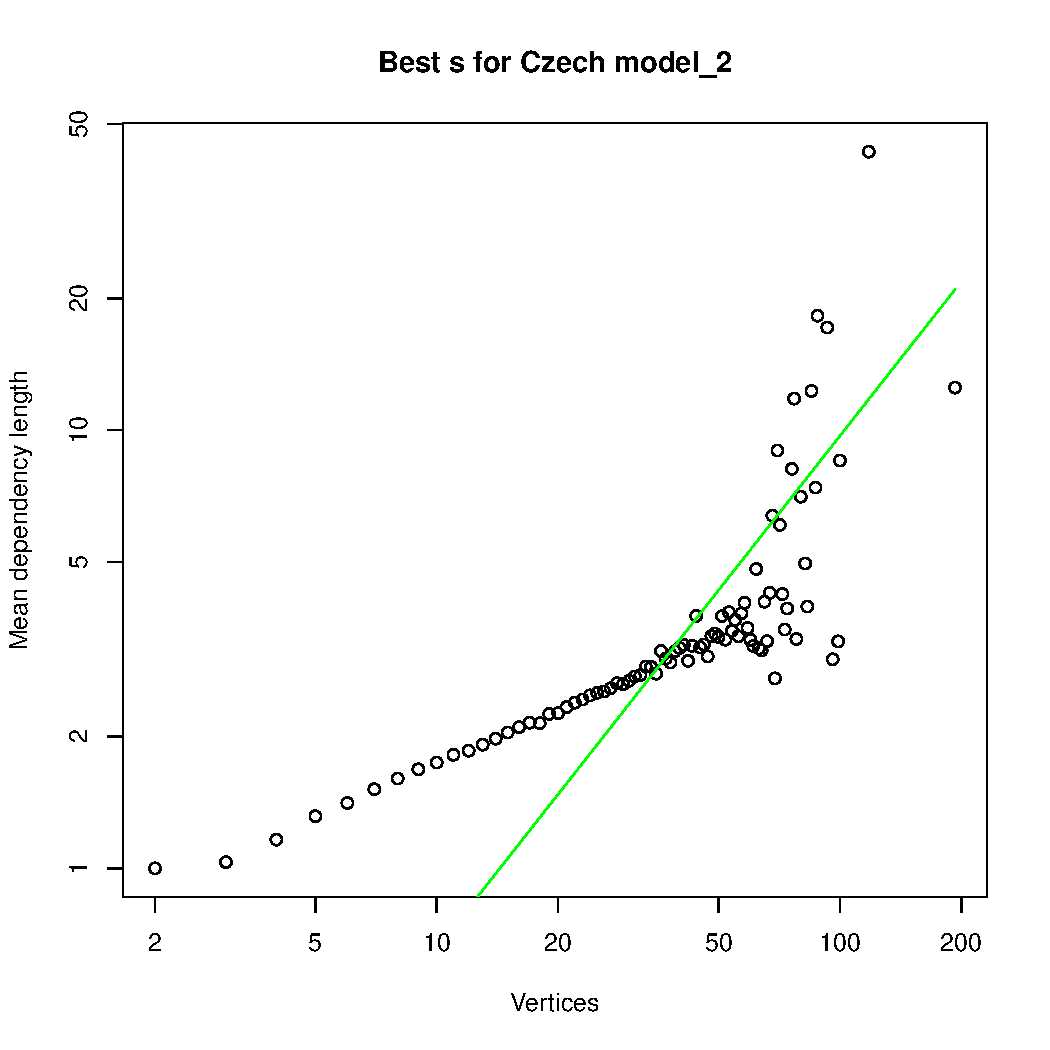
\includegraphics[width=\textwidth]{figures/Czech_best_s.pdf}
        \caption{Model with smallest AIC for Czech.}
        \label{fig:czech_best_aic}
    \end{subfigure} \hfill
    \begin{subfigure}{0.4\textwidth}
        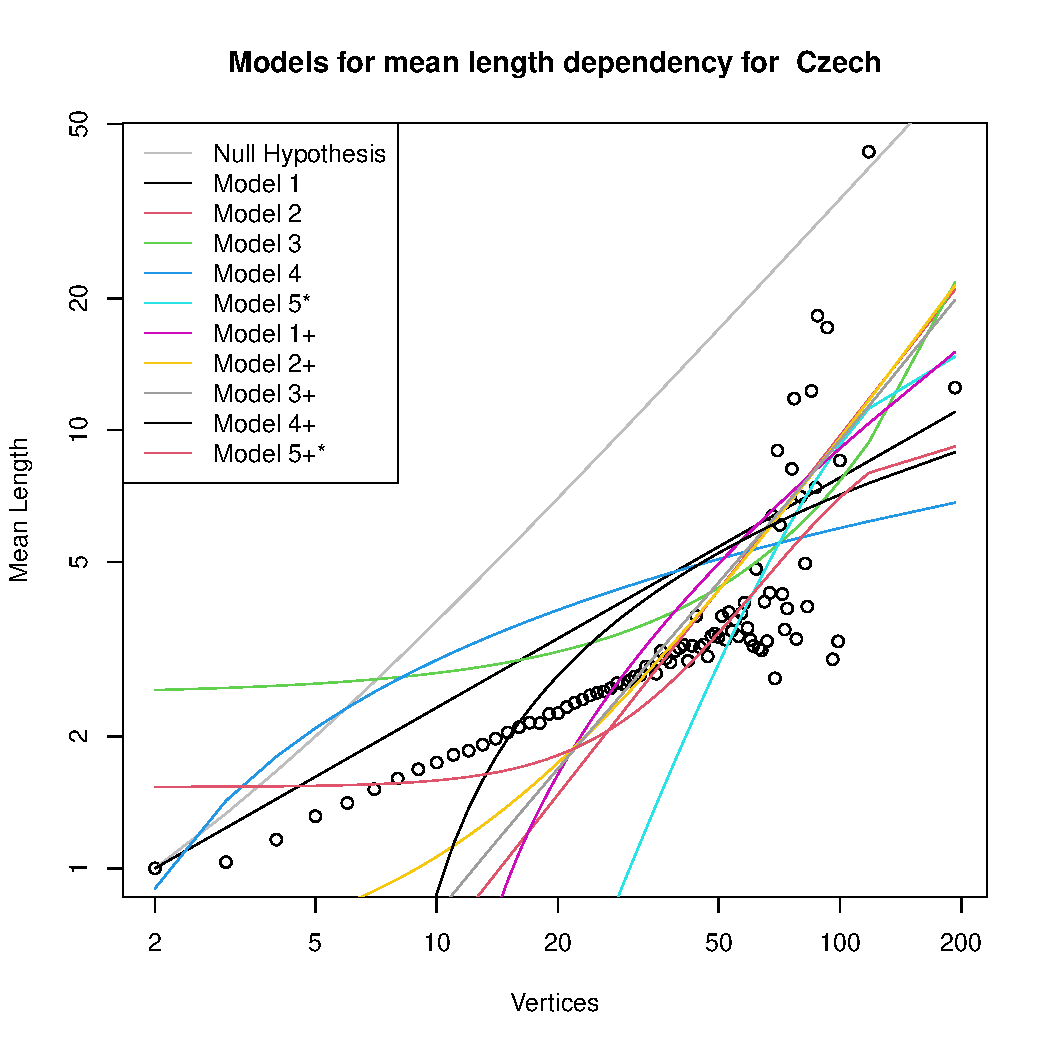
\includegraphics[width=\textwidth]{figures/Czech_all_models.pdf}
        \caption{Models fitted for language Czech.}
        \label{fig:czech_all}
    \end{subfigure}
    \caption{Models fitted for language Czech}
    \label{fig:czech}
\end{figure}

There could several reasonable explanations: either none of the models are good to explain the relation between the number of vertices and the mean length or our optimising method is not appropriate. In Appendix \ref{appendix:weighted}, we show the results of a possible solution in which we weight the samples with the following function $\omega(n) = \frac{1}{n}$. We observe that all the models fit the lower values of the number of vertices better; however, the model with the smallest AIC for Czech still has the same issue, though there is an improvement.We were unable to determine if our weight function $\omega(n)$ was suitable or if we still lacked an adequate model. Our intuition, however, suggests that the weight function could be further enhanced.

\subsection{Extent to which languages resemble or differ}

When visually checking the best models in the appendix \ref{appendix:best-model-plots}, we could separate into two groups: those languages for which the model resembles the behaviour and those for which it differs. The models resemble to Basque, English, Greek, Hungarian, and Turkish. The models differ for Arabic, Catalan, Chinese, Czech, and Italian. We could observe the fact that was mentioned in the previous section that the models fail to resemble the languages when the mean length is really spread for large values of number of vertices. We tried to explain this split using the table \ref{tab:summary}, but there is no clear explanation.

% latex table generated in R 4.3.2 by xtable 1.8-4 package
% Wed Nov 22 15:27:58 2023
\begin{table}[ht]
\centering
\begin{tabular}{lllll}
  \hline
Network & Vertices & Edges & Mean.Degree & Density \\ 
  \hline
Karate & 34 & 78 & 4.5882 & 0.139 \\ 
  Barabasi-Albert & 200 & 800 & 8 & 0.0402 \\ 
  ENRON & 182 & 2097 & 23.044 & 0.1273 \\ 
  DBLP & 2130 & 4587 & 4.307 & 0.002 \\ 
   \hline
\end{tabular}
\caption{Summary of the properties of the networks used.}
\label{tab:summary}
\end{table}


\subsection{Conclusions}

To summarize, it is concluded that the alternative hypothesis models are a good approach to fit the $\langle  d \rangle$ distribution, in comparison with the null hypothesis model.

In addition, it was observed that model 1 was the one providing the best fit for many languages, in particular for half of them, this is due to the fact that the distribution of the values for most of them is linear in the double logarithmic scale, which is what the model 1 and model 2 approach better.

Finally, we suggest a further improvement of the weighted function approach described in \ref{discussion:bestfit}.